\documentclass[a4paper,11pt]{jsbook}

% 目次リンク
\usepackage[dvipdfmx]{hyperref}
\usepackage{pxjahyper}
% 数式
\usepackage{amsmath,amsfonts}
\usepackage{bm}
% 画像
\usepackage[dvipdfmx]{graphicx}
\usepackage[dvipdfmx]{color}

\begin{document}

\title{Splatoon}
\author{さとうあずき}
\date{\today}
\maketitle
\tableofcontents


\chapter{最初の一歩}
\section{コントローラーの操作}
ZRでメインウェポンで攻撃ができる。Lスティックでキャラクターを移動できる。
\begin{figure}[h]
  \begin{center}
    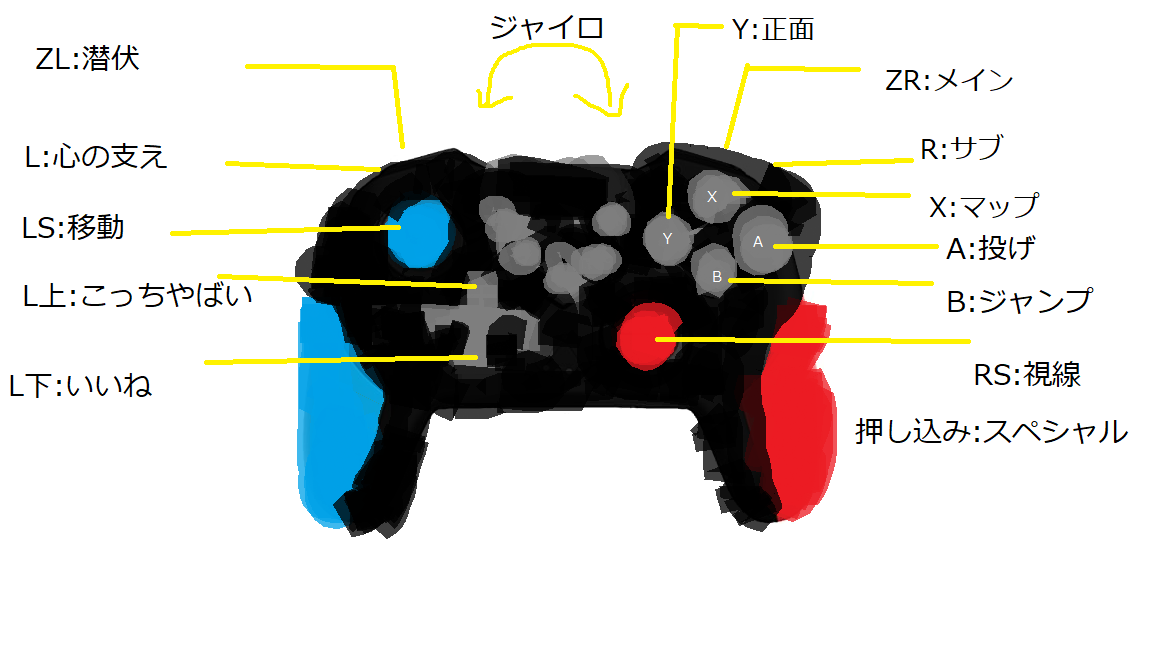
\includegraphics[width=10cm]{resoource/Controller_button.png}
  \end{center}
\end{figure}

試合画面
上に味方と敵のイカマークがある。敵味方の存命がわかる。
右上にスペシャルゲージがある。たまったら、Rスティック押し込みでスペシャルウェポンが使える。
画面中心にレティクルがある。この中に敵を入れてメインウェポンで狙える。ZRでメインウェポンで倒せる。
\begin{figure}[h]
  \begin{center}
    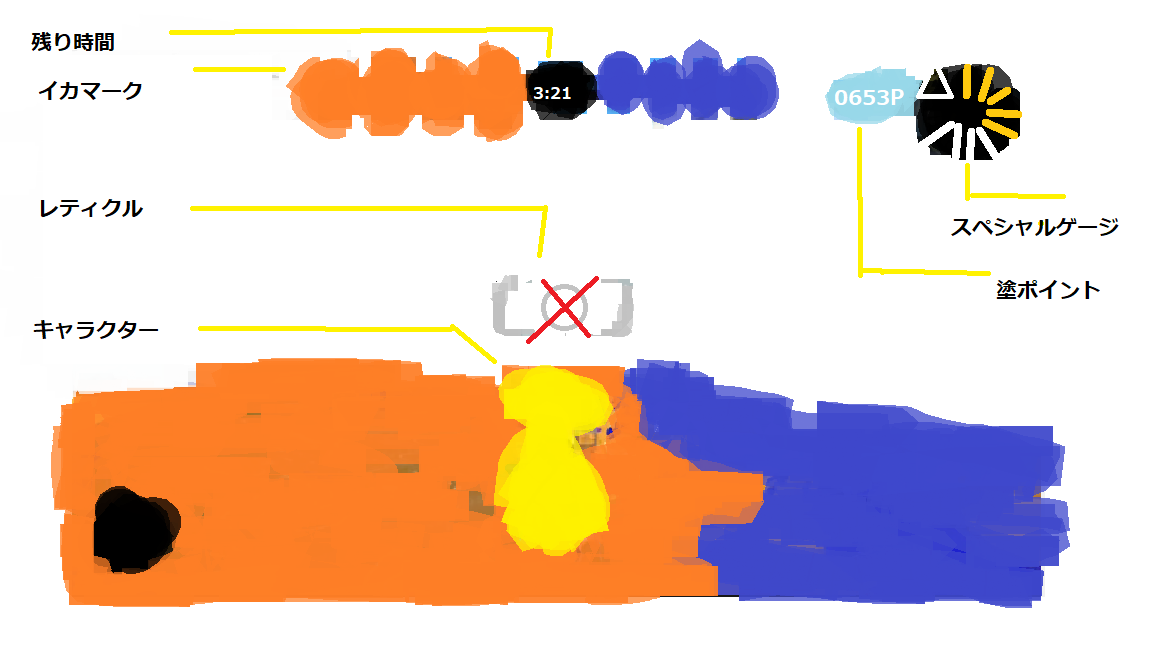
\includegraphics[width=10cm]{resoource/gamescreenframe.png}
  \end{center}
\end{figure}
\section{敵の倒し方}
\subsection{敵との位置関係}
同じ射程の武器同士ではどう戦うべきか。
同じ射程で打ち合い始めて相手に弾が当たらなかったとき移動するべきだろうか
簡単に2次元で敵と対面した時の状況を考える。
\begin{figure}[h]
  \begin{center}
    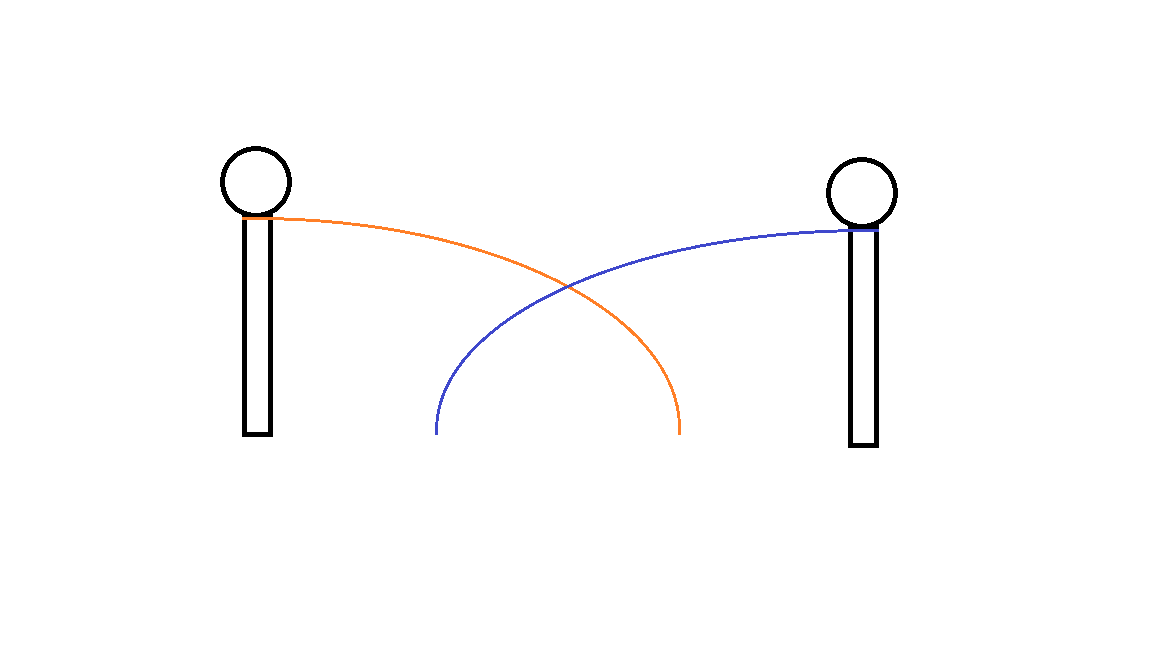
\includegraphics[width=10cm]{resoource/samerange.png}
  \end{center}
\end{figure}

同じ射程で打ち合い始めて相手に弾が当たらなかったとき近づくとどうなるか。
実は、打ち合いに負けてしまう。
自分が近づくと、相手がすでに撃っている弾に自分からあたりに行くことになる。
一方で、自分の弾は近づいて撃ち始めた所で相手にはまだ届いていない。
その結果、先にダメージがたまるのは自分になってしまう。
\begin{figure}[h]
  \begin{center}
    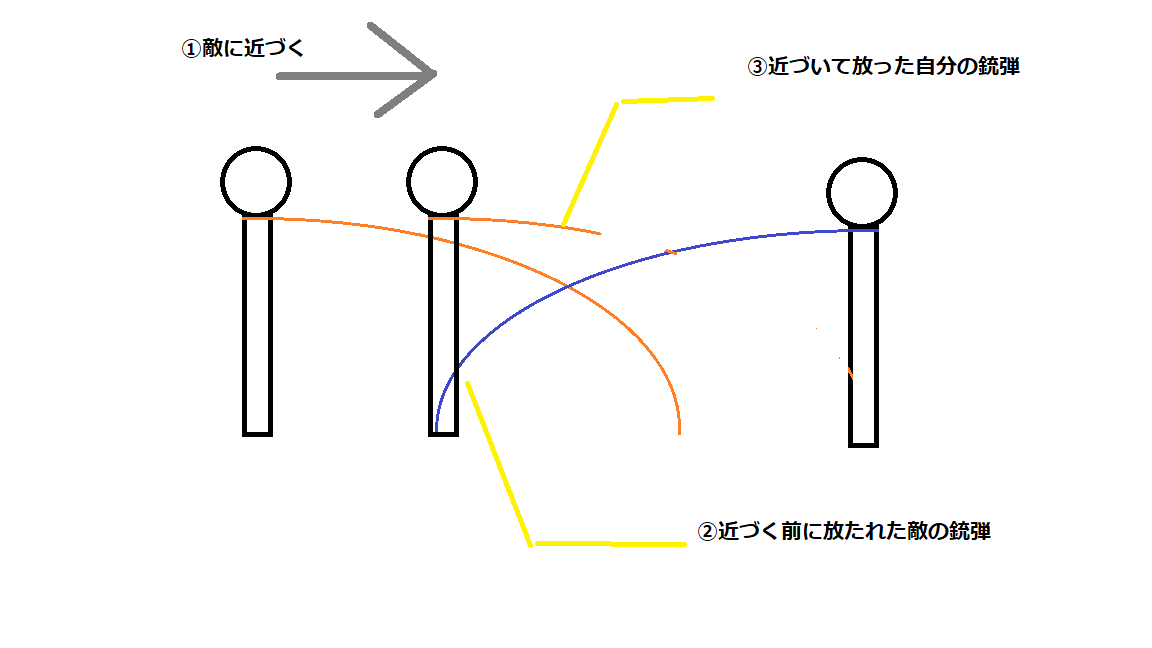
\includegraphics[width=10cm]{resoource/samerange_attacking.png}
  \end{center}
\end{figure}

相手が自分より長射程の武器場合で、打ち合い始めて相手に弾が当たらなかったとき移動するべきだろうか
同様に簡単に2次元で考える。
先ほどと同じように、自分が近づくと、相手がすでに撃っている弾に自分からあたりに行くことになる。
一方で、自分の弾は近づいて撃ち始めた所であっても相手に届くことにはならないだろう。
その結果、先にダメージがたまるのは自分になってしまう。
\begin{figure}[h]
  \begin{center}
    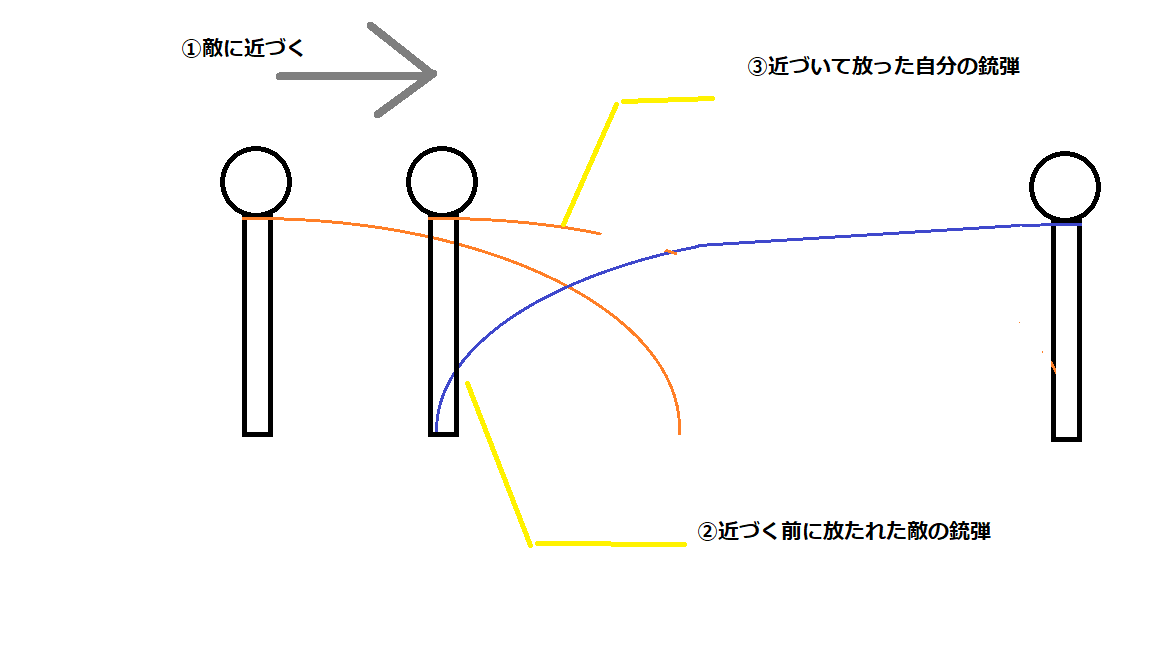
\includegraphics[width=10cm]{resoource/long_range_attacking.png}
  \end{center}
\end{figure}


相手が自分より短射程の武器場合で、打ち合い始めて相手に弾が当たらなかったとき移動するべきだろうか
同様に簡単に2次元で考える。
先ほどと同じように、自分が近づくと、自分の弾が先に相手に当たる所がある。
その結果、先にダメージがたまるのは敵になる。
しかし、自分の弾が先に相手に当たる所よりさらに近づくと、相手がすでに撃っている弾に自分からあたりに行くことになる。

\begin{figure}[h]
  \begin{center}
    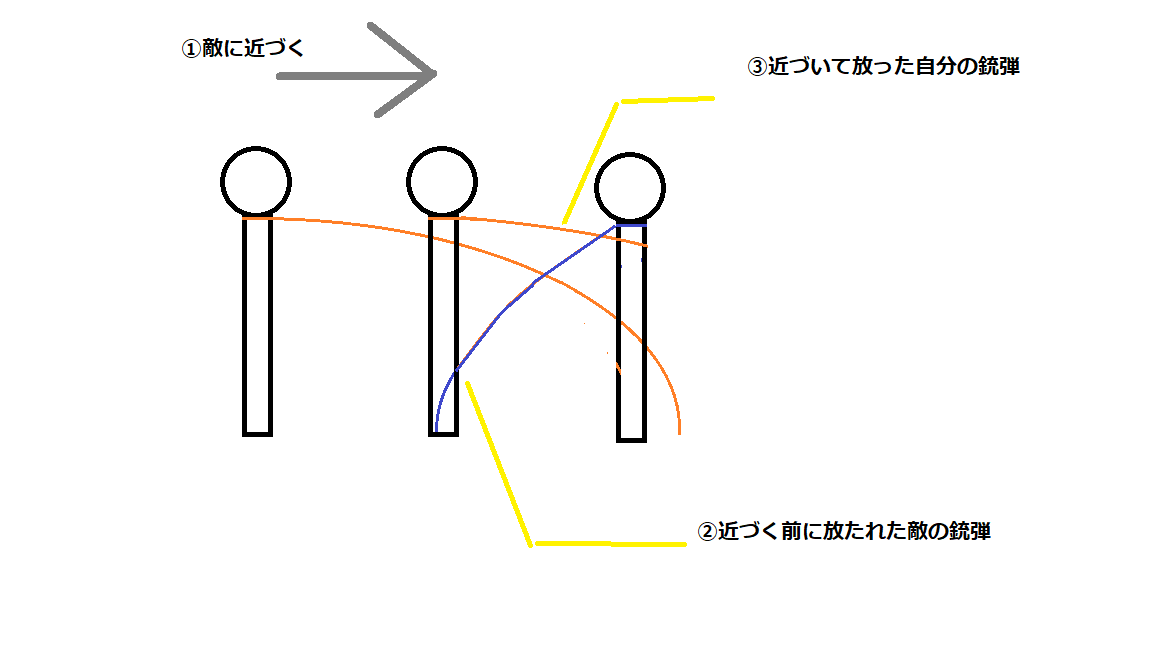
\includegraphics[width=10cm]{resoource/short_range_attacking.png}
  \end{center}
\end{figure}

以上から、2次元平面内で敵に近づくという戦術はよくない。
自分の射程以上に長い相手には近づくとやられる。
自分が相手より射程が長いときは、相手の射撃が当たらない位置まで近づくことはできるが、それ以上近づくと負ける要素が出てくる。
もちろん、実際のゲームは3次元で行われる。武器も単位時間あたりの弾の数が異なるし、弾当たりのダメージも異なる。プレイヤーは逃げ回るし、狙う対象ががプレイヤーとも限らない。
このような要素から勝負の駆け引きは発生するが、基本的に射程が届かない相手を倒すことはできない。自分の射程と相手の射程を念頭に勝負を始めよう。

相手を倒そうと意気込むだけで相手に近づくのは悪手であることが多い。\footnote{諸。敵に何度もやられようが正面から何度も突っ込みまくるプレイヤー。猪の対義語に芋がある。}
諸突猛進するプレイヤーが悪いとは思わない。ただし、プレイヤーが持つ戦術が猪しかないというのは心もとない。
じゃんけんでグーしか出さないという戦術を進んで行う人はいないだろう。

\subsubsection{射程の暴力}
敵の倒し方からわかるように、長い射程のほうが勝負を有利に進められる。長い射程であれば敵から攻撃を受けることなく一方的に敵を蹂躙し、試合に勝つことができてしまう。
これを射程の暴力と呼ぶ人もいる。
シューティングゲームでは、長射程武器を持つ敵をどうやって倒すかがとても大事になってくる。

\subsection{敵との距離の詰め方}
敵と対面した位置関係について2次元的に考えたところ、結局近づかないことが有利であることが分かった。
しかし、自分の武器の射程範囲に敵がいなければ敵を打ち倒すことはできない。
この小節では敵との距離をどう詰めるかについて考えてみる。
\subsubsection{敵に近づく}


\subsubsection{敵が近づく}

\subsection{敵を撃つやり方}




\chapter{初めに}
\section{Splatoon}
\subsection{ゲームが目指しているところ}
人は目が覚めたらご飯を食べ、トイレに行き、将来に向けてあくせくと働き、そして寝る。
最適化された生活の中には喜怒哀楽もなく、ただ平然と人生を消費していき、死ぬ。
最適化された生活から脱却するような無駄な行為である。
しかし、人生において無駄な行為こそ、人生を謳歌するための唯一の手段である。
人生においてゲームは必要ない。だからこそゲームの中での一喜一憂は我々の生活を豊かにし、そして生まれた意味になる。

\subsection{Splatoon3とは}
Splatoon3は2022年9月8日に任天堂から発売開始され、発売3日間で国内販売本数345万本を記録した大人気ゲームソフトである。
このゲームはイカやタコが4対4のチームを組み、インクを垂らしながら陣地を奪ったりルールに基づいてポイントを稼いだりして勝敗を決める、新感覚のシューティングゲームである。
老若男女問わず楽しめるもので初心者からプロもプレイし、このゲームを通して世界中のプレイヤーはゲームのランキングを競いあっている。

\subsection{Splatoonへの憤り}
Splatoonは大変面白いゲームであり、世界中から愛されている。
素晴らしいプレイがあれば喜び、強い敵に打ち負かされて悲しみ、このゲームを通して我々は充実した時間を過ごすことができるだろう。
しかし、Splatoonをこよなく愛するプレイヤーの中にはどうやらただただストレスをうけ、さらにそのプレイヤーの罵声や怒号によって周りの人間を不愉快にさせ、何のためにゲームをやっているのかわからなくなっている人がいるようだ。
私はそんな人たちが少しでも充実したゲーム人生を過ごしてもらうと、筆を執ることにした。


\section{ゲームを楽しむ}


\subsection{勝負に勝つ}


\subsection{試合に勝つ}





\chapter{試合を優位に進める}
\section{大局的人数有利}
\subsection{通信障害}
\subsection{イカマーク}
\subsection{マッチルールオブジェクト}
マッチルールオブジェクトを味方と考える。→三角関係

\section{局所的人数有利}
\subsection{三角関係}
自分と相手と何か
味方
ルール関与オブジェクト
自分の残像



\subsection{戦線}
敵と味方が打ち合っている境界線
\begin{figure}[h]
  \begin{center}
    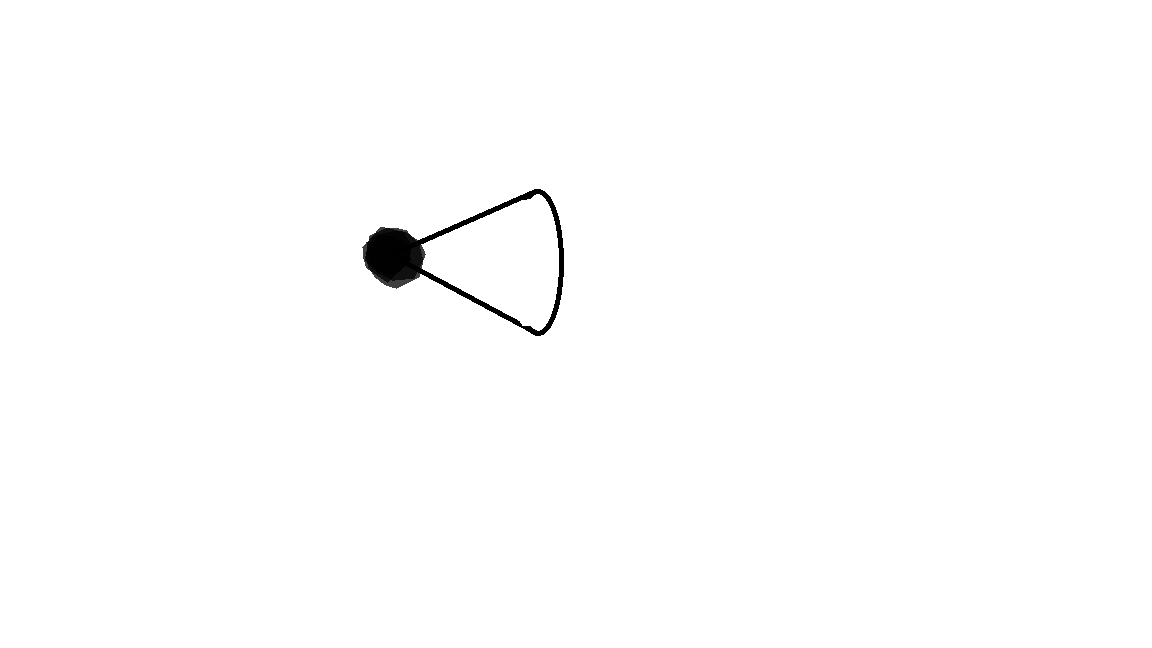
\includegraphics[width=10cm]{resoource/player.png}
  \end{center}
\end{figure}

\subsection{前線}
戦線にヘルプに入れる位置で自陣のリスボーンに一番近い位置

\section{地形有利}
\subsection{高所}
相手の位置がわかる、自分の位置は相手はわからない

\subsection{オブジェクト}
\section{チーム構成有利}
\subsection{スペシャルウェポン有利}
打開
射程
\subsection{サブウェポン有利}
打開
射程
\subsection{メインウェポン有利}
打開
射程
\subsection{ギア有利}
打開
射程

\chapter{勝負を優位に進める}
\section{メインウェポン}
\subsection{射程と索敵}
\subsection{射程とキル}
\section{サブウェポン}
\subsection{索敵}
\section{スペシャルウェポン}
\section{イカ状態とヒト状態}
\subsection{当たり判定}
ヒト状態とイカ状態
右打ち
\subsection{インク回復}
\subsection{移動速度}
\subsection{インク潜伏}
\section{マップ}
\section{キャラクター移動}
\subsection{風神雷神}
\section{スーパージャンプ}
\section{ジャンプ}
\section{やられたとカモンとナイス}
\section{カメラリセット}

\chapter{ガチマッチで勝つ}
\section{ガチエリア}
\subsection{カウントを進める}
マッチルールオブジェクトと前線、戦線
マッチルールオブジェクトはエリアになり、エリアはステージ中心に存在する。
オブジェクト付近に敵を近づけさせないために、前線はステージ中心より敵陣側
前線と敵陣リスポーンの間に戦線が発生する

\subsection{カウントを奪う}
マッチルールオブジェクトと前線、戦線
マッチルールオブジェクトはエリアになり、エリアはステージ中心に存在する。
オブジェクト付近に近づくために、前線がステージ中心にある
戦線と自陣リスポーンの間に前線が発生する


\section{ガチヤグラ}
\section{ガチホコ}
\section{ガチアサリ}


\chapter{謝辞}

\appendix
\chapter{A}



\begin{thebibliography}{2}

\bibitem{K.miyuki}K.miyuki (private communication)
\end{thebibliography}

\thispagestyle{empty}
\vspace*{\stretch{1}}
\begin{flushright}
\begin{minipage}{0.5\hsize}
\begin{description}
  \item{著者:}さとうとーま
  \item{挿絵:}さとうとーま
  \item{発行:}\date{\today}
  % \item{印刷:}POPLS (\verb|http://www.inv.co.jp/~popls/|)
\end{description}
\end{minipage}
\end{flushright}

\end{document}











